\documentclass[svgnames]{beamer}
\usetheme{Warsaw}
\usepackage{xcolor}
\usepackage{graphicx}
\usepackage{emoji}

\beamertemplatenavigationsymbolsempty

\addtobeamertemplate{navigation symbols}{}{%
    \usebeamerfont{footline}%
    \usebeamercolor[fg]{footline}%
    \hspace{1em}%
    \insertframenumber/\inserttotalframenumber
}

\title{Notes de la vie}
\subtitle{1ère édition} 
\author{Comité pour les notes de la vie}
\date{Q1 2023}

\begin{document}

\maketitle

\section{Introduction}

\begin{frame}{Quelques chiffres...}
    \begin{itemize}
        \item <1-> \textbf{11} participants
        \item <2-> \textbf{13} semaines
        \item <3-> \textbf{1} note par semaine entre \textbf{0} et \textbf{10}
        \item <4-> ... \textbf{143} notes !
    \end{itemize}
\end{frame}

\begin{frame}{Le concept}
    \centering
    La note de la semaine reflète la \textbf{qualité} de la semaine passée et la \textbf{psyché} d'une personne. Elle est à la fois \textbf{synthèse} et \textbf{sentiment}.
\end{frame}

\begin{frame}{Rigueur scientifique}

\begin{alertblock}{Retards}
De multiples \textbf{retards} ont été constatés. Cela à considérablement porté atteinte à la \textbf{crédibilité} du projet.
\end{alertblock}
    
\end{frame}

\section{Le jus de données}

\begin{frame}{Trajectoires de vie}

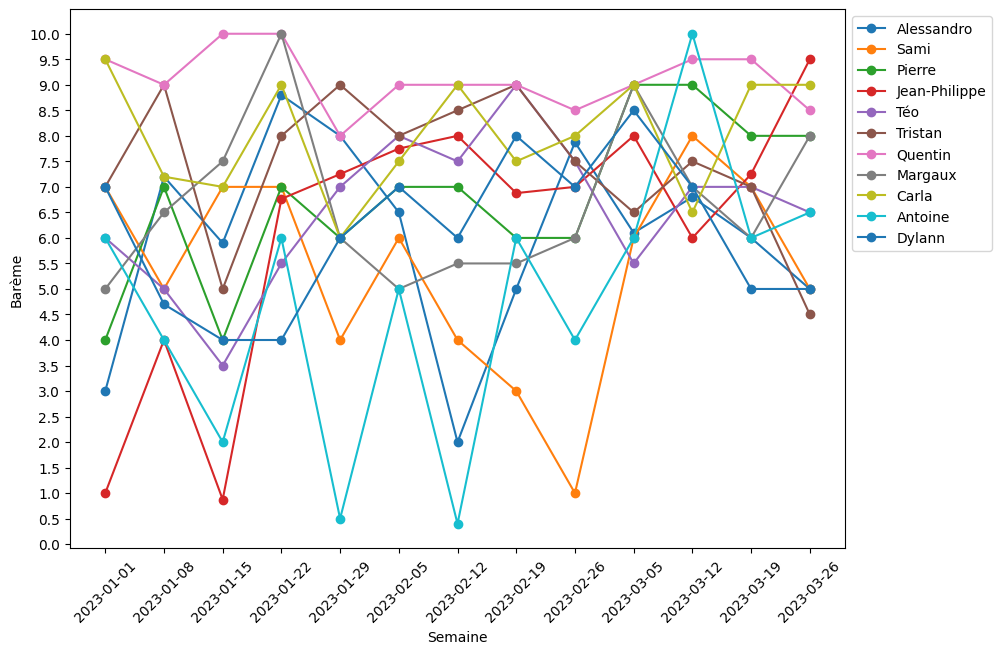
\includegraphics[width=\textwidth]{data/plot.png}
    
\end{frame}

\begin{frame}{Des vies différentes}

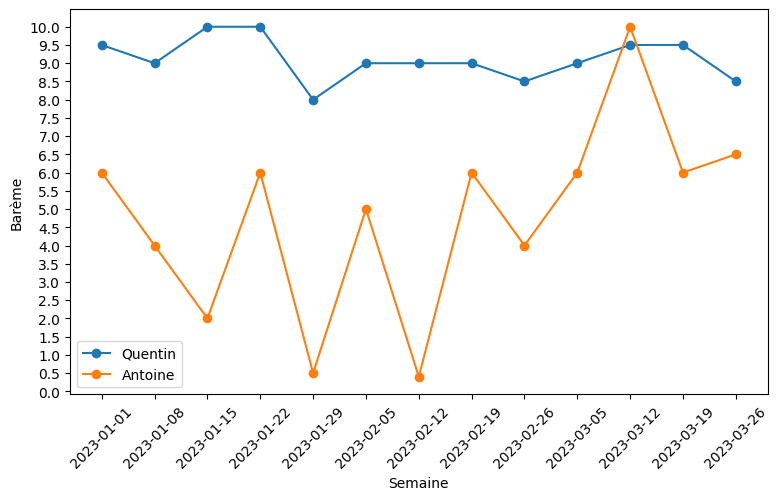
\includegraphics[width=\textwidth]{data/quentin_antoine.png}
    
\end{frame}

\begin{frame}{Des boîtes et des moustaches}

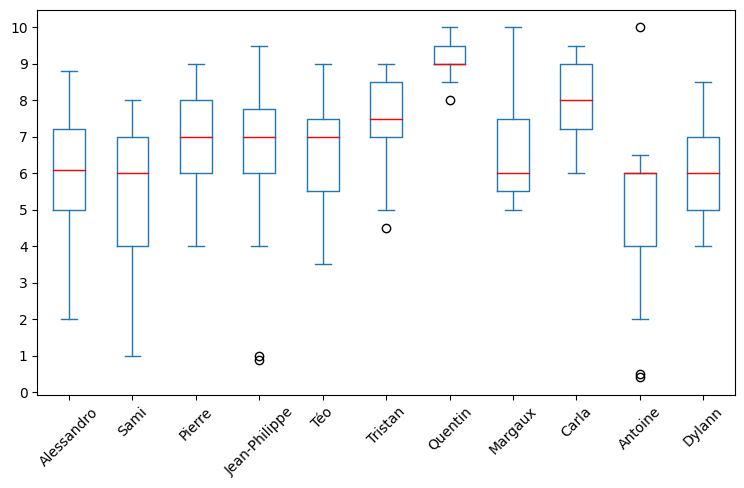
\includegraphics[width=\textwidth]{data/box_plot.png}
    
\end{frame}

\begin{frame}{Les violons c'est mieux}

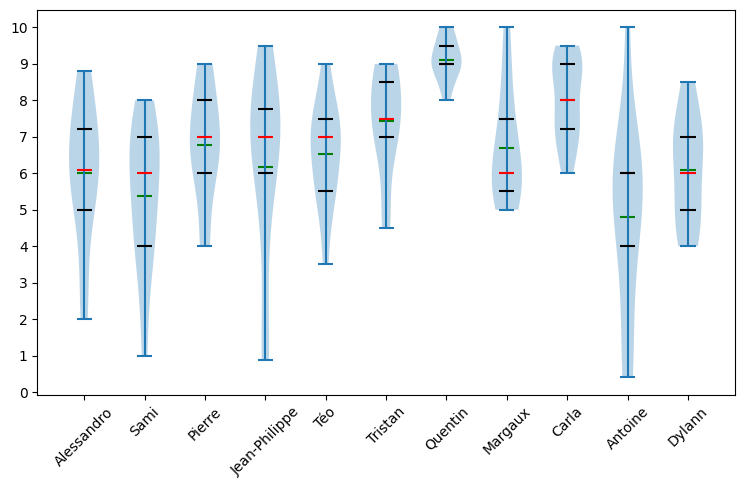
\includegraphics[width=\textwidth]{data/violin_plot.png}
    
\end{frame}

\begin{frame}{Des hauts et des bas}

\begin{table}[!ht]
    \centering
    \begin{tabular}{|l|l|}
    \hline
        ~ & \textbf{Écart type} \\ \hline
        Antoine & 2.648 \\ \hline
        Jean-Philippe & 2.640 \\ \hline
        Sami & 1.981 \\ \hline
        Alessandro & 1.930 \\ \hline
        Pierre & 1.589 \\ \hline
        Margaux & 1.548 \\ \hline
        Dylann & 1.467 \\ \hline
        Tristan & 1.441 \\ \hline
        Téo & 1.436 \\ \hline
        Carla & 1.142 \\ \hline
        Quentin & 0.583 \\ \hline
    \end{tabular}
\end{table}
    
\end{frame}

\begin{frame}{Le classement officiel}

\begin{table}[!ht]
    \centering
    \begin{tabular}{|l|l|l|}
    \hline
        ~ & \textbf{Score /130} & \textbf{Score \%} \\ \hline
        Quentin \emoji{1st-place-medal} & 118.5 & 91.15 \\ \hline
        Carla \emoji{2nd-place-medal} & 104.2 & 80.15 \\ \hline
        Tristan \emoji{3rd-place-medal} & 96.5 & 74.23 \\ \hline
        Pierre & 88.0 & 67.69 \\ \hline
        Margaux & 87.0 & 66.92 \\ \hline
        Téo & 85.0 & 65.38 \\ \hline
        Jean-Philippe & 80.26756 & 61.74 \\ \hline
        Dylann & 79.2 & 60.92 \\ \hline
        Alessandro & 78.175 & 60.13 \\ \hline
        Sami & 70.0 & 53.85 \\ \hline
        Antoine & 62.4 & 48.0 \\ \hline
    \end{tabular}
\end{table}
    
\end{frame}

\begin{frame}{Le gâteau}

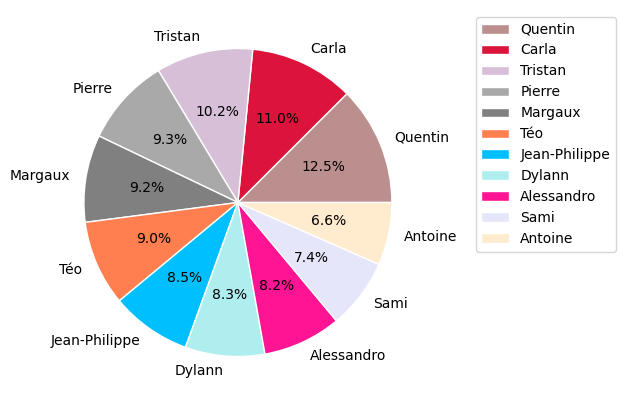
\includegraphics[width=\textwidth]{data/pie.png}
    
\end{frame}

\begin{frame}{- Quelle semaine hein ? - Capitaine on est mercredi...}
    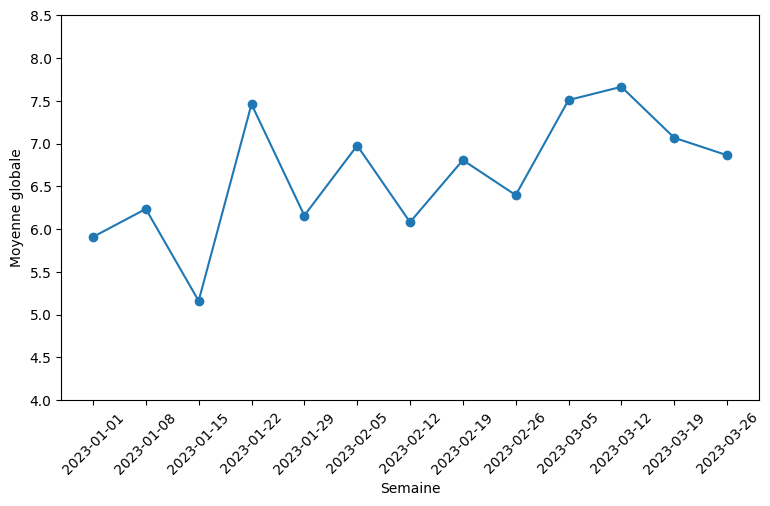
\includegraphics[width=\textwidth]{data/semaines.png}
\end{frame}

\section{Conclusion}

\begin{frame}{Je suis à votre écoute}
    \begin{itemize}
    \item <1-> Est-ce que vous avez aimé l'expérience ?
    \item <2-> Est-ce que vous voulez continuer ?
    \item <3-> Est-ce que vous voulez changer quelque chose ?
\end{itemize}
\end{frame}

\begin{frame}{Passation de pouvoir}

\begin{figure}
    \centering
    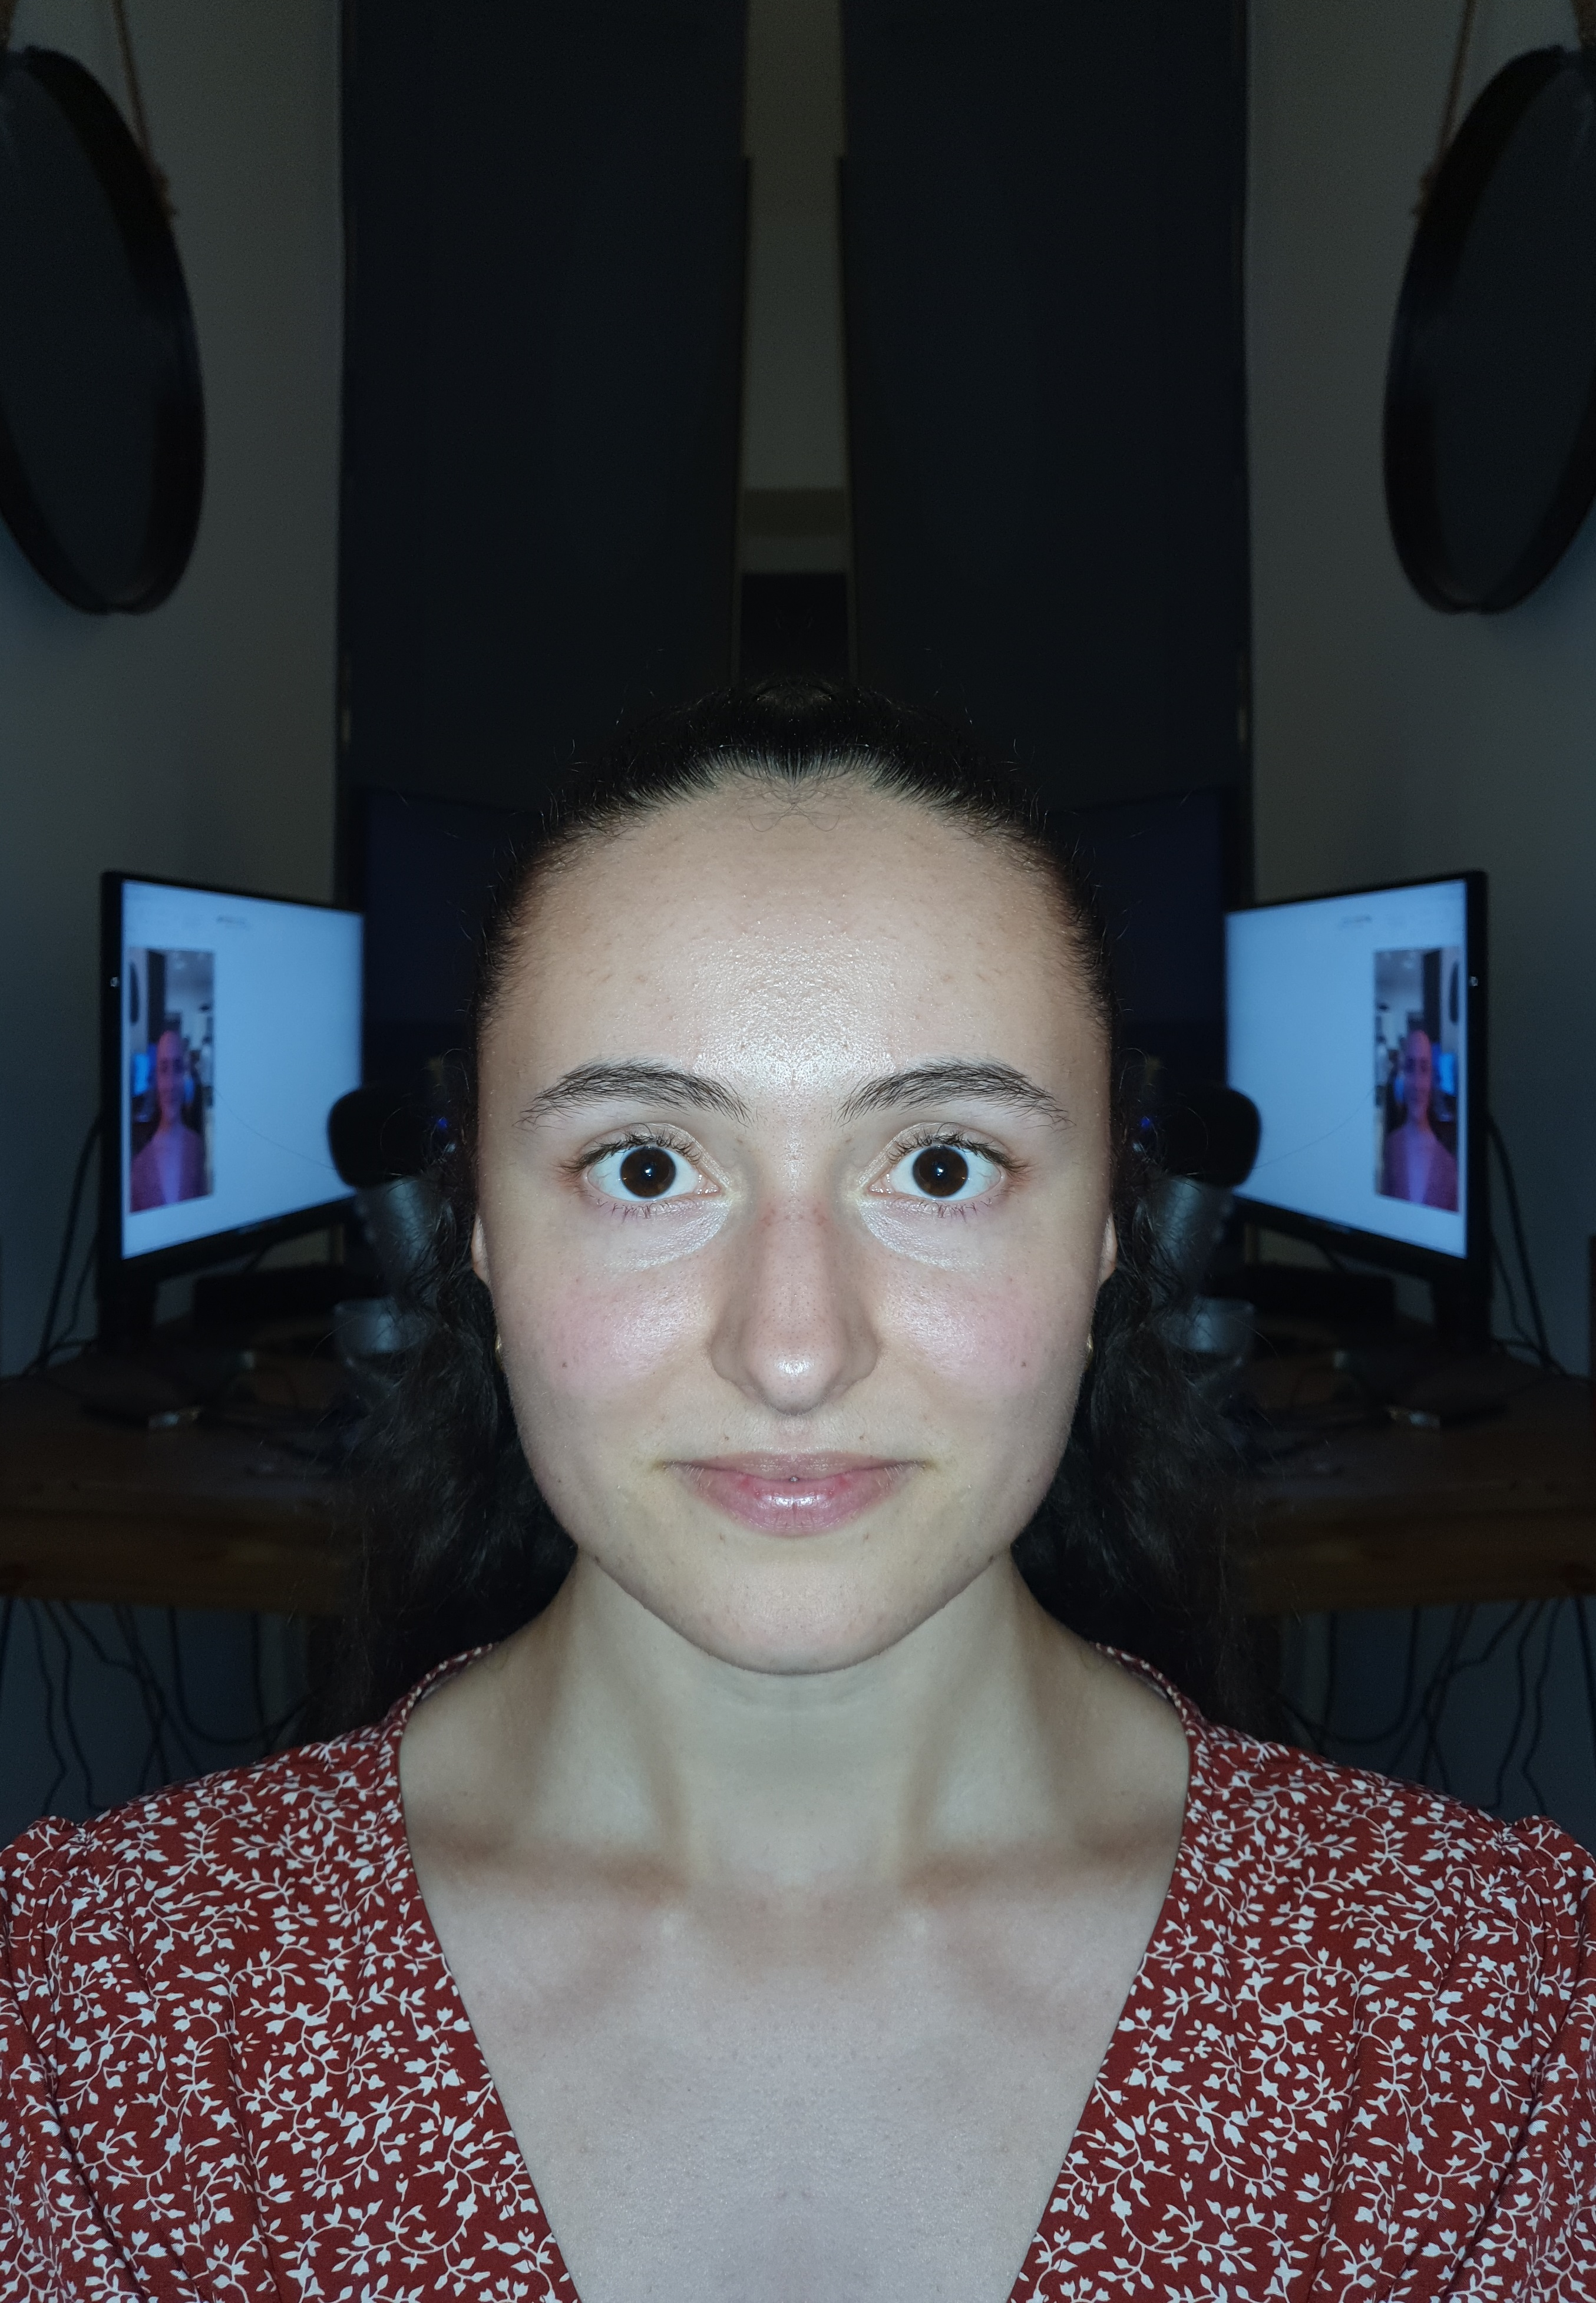
\includegraphics[scale=0.05]{data/carla.jpg}
    \caption{Clara Guerrero (photo non altérée)}
    \label{fig:my_label}
\end{figure}
    
\end{frame}

\begin{frame}{Fin}
    Merci pour votre attention. \emoji{heart} \newline

    Le code est disponible sur GitHub : \newline

    \centering
    \href{https://github.com/Allez100dreau/notesdelavie}{\texttt{https://github.com/Allez100dreau/notesdelavie}}
\end{frame}

\end{document}
